\chapter{Introduction}

\section{On Artificial Intelligence (AI) and Computational Linguistics}
% copied from intro
In 1950 Alan Turing in a seminal paper \citep{Turing1950} published in Mind was asking if ``machines can do what we (as thinking entities) can do?'' He questioned what intelligence was and whether it could be manifested in machine actions indistinguishable from human actions. 

He proposed the famous \textit{Imitation Game} also known as the \textit{Turing test} in which a machine would have to exhibit intelligent behaviour equivalent or indistinguishable from that of a human. The test was set up by stating the following rules. The machine (player A) and a human (player B) are engaged in a written \textit{natural language} conversation with a human judge (player C) who has to decide whether each conversation partner is human or a machine. The goal of players A and B is to convince the judge (player C) that they are human. 

This game underpins the question whether ``a computer, communicating over a teleprinter, (can) fool a person into believing it is human?'', moreover, whether it can exhibit (or even appear to exhibit) human(-like) cognitive capacities \citep{Harnad1992}. Essential parts of such cognitive capacities and intelligent behaviour that the machine needs to exhibit are of course the linguistic competences of comprehension (or ``understanding'') and generation of ``appropriate'' responses (for a given input from the judge C).

The \textit{Artificial Intelligence} (AI) field was born from dwelling on Turing's questions. The term was coined by McCarthy for the first time in 1955 referring to the ``science and engineering of making intelligent machines'' \citep{McCarthy1955}.

The general target is to program machines to do with language what humans do. Various fields of research contribute to this goal. Linguistics, amongst others, contributes with theoretical frameworks systematizing and accounting for language in terms of morphology, phonology, syntax, semantics, discourse or grammar in general. In computer science increasingly more efficient algorithms and machine learning techniques are developed. Computational linguistics provides methods of encoding linguistically motivated tasks in terms of formal data structures and computational goals. In addition, specific algorithms and heuristics operating within reasonable amounts of time with satisfiable levels of accuracy are tailored to accomplish those linguistically motivated tasks.

\textit{Computational Linguistics} (CL) was mentioned in the 1950 in the context of automatic translation \citep{Hutchins1999} of Russian text into English and developing before the field of Artificial Intelligence proper. Only a few years later CL became a sub-domain of AI as an interdisciplinary field dedicated to developing algorithms and computer software for intelligent processing of text (leaving the very hard questions of intelligence and human cognition aside). Besides \textit{machine translation} CL incorporates a broader range of tasks such as \textit{speech synthesis and recognition, text tagging, syntactic and semantic parsing, text generation, document summarisation, information extraction} and others. 
%New higher level and more complex tasks are formulated in academic and business environments as the simpler ones receive satisfiable 

This thesis contributes to the field of CL and more specifically it is an advancement in \textit{Natural Language Parsing} (NLP), one of the central CL tasks informally defined as the process of transforming a sentence into (rich) machine readable syntactic and semantic structure(s). Developing a program to automatically analyse text in terms of such structures by involving computer science and artificial intelligence techniques is a task that has been pursued for several decades and still continues to be a major challenge today. This is especially so when the target is \textit{broad language coverage} and even more when the desired analysis goes beyond simple syntactic structures and towards richer functional and/or semantic descriptions useful in the latter stages of \textit{Natural Language Understanding} (NLU). The current contribution aims at a reliable modular method for parsing unrestricted English text into a feature rich constituency structure using Systemic Functional Grammars (SFGs). 

In computational linguistics, broad coverage natural language components now exist for several levels of linguistic abstraction, ranging from tagging and stemming, through syntactic analyses to semantic specifications. In general, the higher the degree of abstraction, the less accurate the coverage becomes and, the richer the linguistic description, the slower the parsing process is performed. 

Such working components are already widely used to enable humans to explore and exploit large quantities of textual data for purposes that vary from the most theoretical, such as understanding how language works or the relation between form and meaning, to very pragmatic purposes such as developing systems with natural language interfaces, machine translation, document summarising, information extraction and question answering systems to name just a few. 

%end copied from intro

\section{Living in technologically ubiquitous world}
\label{sec:motivation}
Developed over thousands of years, the human language has become a versatile highly nuanced form of communication that carries a wealth of meaning which by far transcends the words alone. When it comes to \textit{human-machine} interaction this highly articulated communication form is deemed impractical. So far humans had to learn to interact with computers and do it in  formal, strict and rigorous manner via graphical user interfaces, command line terminals and programming languages. Advancements in \textit{Natural Language Processing} (NLP) which is a branch of \textit{Artificial Intelligence} (AI) are a game changer in this domain. NLP starts to unlocks the information treasure locked in the human speech and make it available for processing to computers. NLP becomes an important technology in bridging the gap between natural data and digital structured data.

In a world such ours, where technology is ubiquitous and pervasive in almost all aspects of our life, NLP becomes of great value and importance regardless whether it materializes as a spell-checker, intuitive recommender system, spam filter, (not so) clever machine translator, voice controlled car, intelligent assistants such as Siri, Alexa or Google Now. 

Every time you ask Siri or Alexa for directions to the nearest Peruvian restaurant, how to cook Romanian beef stew or what is the dictionary definition for the word \textit{germane}, a complex chain of operations is activated that allows `her' to understand the question, search for the information you are looking for and respond in a human understandable language. Such tasks are possible only in the past few years thanks to advances in NLP. Until now we have been interacting with computers in a language they understand rather than us. Now they are learning our language. 

\section{NLP for businesses}
\label{sec:motivation-business}
NLP opens new and quite dramatic horizons for businesses. Navigating with limited resources stormy markets of competitors, customers and regulators and finding an optimal answer/action to a business question is not a trivial task. 
Markets are influenced by the information exchange and being able to process massive amounts of text and extract meaning can help asses the status of an industry and play an essential role in crafting a strategy or a tactical action. 
Relevant NLP tasks for gathering market intelligence are \textit{named entity recognition} (NER), \textit{event extraction} and \textit{sentence classification}. With these tasks alone one can build a database about companies, people, governments, places, events together with positive or negative statements about them and run versatile analytics to audit the state of affairs.

Compliance with governmental, European or international regulations is a big issue for large corporations. One question for addressing this problem is whether a product is a liability or not and if yes then in which way. Pharma companies for example, once a drug has been released for clinical trials, need to process the unstructured clinical narratives or patient's reports about their health and gather information on the side effects. The NLP tasks needed for this applications are primarily \textit{NER} to extract names of drugs, patients and pharma companies and \textit{relation detection} used to identify the context in which the side effect is mentioned. NER task help transforming a sentence such as ``Valium makes me sleepy'' to ``(drug) makes me (symptom)'' and relation detection will apply patterns such as ``I felt (symptom) after taking (drug)'' to detect the presence of side effects.

Many customers, before buying a product, check online reviews about the company and the product whether it is pizza or a smartphone. Popular sources for such inquiry are the blogs, forums, reviews, social media, reports, news, company websites, etc. All of them contain a plethora of precious information that stays trapped in unstructured human generated text. This information if unlocked can play a great deal in company's reputation management and decisions for necessary actions to improve it. The NLP tasks sufficient to address this business required are \textit{sentiment analysis} to identify attitude, judgement, emotions and intent of the speaker, and \textit{co-reference resolution} which connects mentions of things to their pronominal reference in the following or preceding text. These tasks alone can extract the positive and negative attitudes from sentence ``The pizza was amazing but the waiter was awful!'' and connect it to the following sentence ``I adore when it is topped with my favourite artichoke'' about pizza and not the waiter and discover a topping preference.

NLP is heavily used in customer service in order to figure out what customer means not just what she says. Interaction of companies with their customers contain many hints pointing towards their dissatisfaction and interaction itself is often one of the causes. Companies record, transcribe and analyse large numbers of call recordings for extended insights. They deploy chat bots fo increased responsiveness by providing immediate answers to simple needs and also decrease the load of the help desk staff. NLP tasks that are essential in addressing some of the customer service needs are \textit{speech recognition} that converts speech audio signal into text and \textit{question answering} which is a complex task of recognising the human language question, extract the meaning, searching relevant information in a knowledge base and generate an ineligible answer. Advances in deep learning allow nowadays to skip the need for searching in a knowledge base by learning from large corpora of question-answer pairs complex interrelations. 

The above cases underline the increased need in NLP whereas the variation and ever increasing complexity of tasks reveal the need in deeper and richer semantic and pragmatic analysis across a broad range of domains and applications. Any analysis of text beyond the formal aspects such as morphology, lexis and syntax inevitably lead to a functional paradigm of some sort which can be applied not only at the clause level but at the discourse as a whole. This makes the text also an artefact with relation socio-cultural context where it occurs. 

\section{The linguistic framework}
\label{sec:framework}
Any description or analysis involving language implies some theory of about its essential nature and how it works. A linguistic theory includes also goals of linguistics, assumptions about which methods are appropriate to approach those goals and assumptions about the relation between theory, description and applications \citep{Fawcett2000}. 

In this thesis I adopt the Systemic Functional Linguistic (SFL) framework because of its versatility to account for the complexity and phenomenological diversity of human language providing descriptions along \textit{multiple semiotic dimensions} i.e. paradigmatic, syntagmatic, meta-functional, stratification and instantiation dimensions \citep{Halliday2003} and at different \textit{delicacy levels} of the \textit{lexico-grammatical cline} \citep{Halliday2002, Hasan2014}. Just like the resolution of a digital photo defines the clarity and the amount of detail in the picture, the same way delicacy refers to the how fine or coarse grained distinctions are made in the description of the language. And intuitively the lexico-grammar is the combination of the lexis and grammar into a single description. These notions and other elements of the SFL theory are addressed below in Chapter \ref{ch:sfg}.

In his seminal paper ``Categories of the theory of grammar'' \citep{Halliday61-orig}, Halliday lays the foundations of SFL following the works of his British teacher J. R. Firth, inspired by Louis Hjelmslev \citep{Hjelmslev53} from Copehagen School of linguistics and by a group of European linguists from Prague Linguistic Circle. This paper constitutes a response to the need for a \textit{general theory of language} that would be holistic enough to guide empirical research in the broad discipline of linguistic science:
\begin{quotation}
    ... the need for a \textit{general} theory of description, as opposed to a \textit{universal} scheme of descriptive categories, has long been apparent, if often unformulated, in the description of all languages \citep[p.54; emphasis in original]{Halliday57}
\end{quotation} 
\begin{quotation}
    If we consider general linguistics to be the body of theory, which guides and controls the procedures of the various branches of linguistic science, then any linguistic study, historical or descriptive, particular or comparative, draws on and contributes to the principles of general linguistics \citep[p.55]{Halliday57}
\end{quotation} 

% deeper on SFL
With this perspective, paradigmatic organization of language received priority as the primary focus of linguistic description and subsequently the structure is analysed as a realisation of features. 

%TODO: use here metrial from Bateman2017-sfl [the place of systemic functional linguistics ... 21 century]

SFL regards language as a social semiotic system where any act of communication is regarded as a conflation of \textit{linguistic choices} available in a particular language. Choices are organised on a paradigmatic rather than structural axis and represented as \textit{system networks}. Moreover, in the SFL perspective language has evolved to serve particular \textit{functions} influencing their the structure and organisation of the language. However, their organisation around the paradigmatic dimension leads to a significantly different functional organisation than those found in several other frameworks which \citet{Butler2003-pt1, Butler2003-pt2} extensively addresses. 

Embracing the \textit{oragnon model} formulated by \citet{Buhler34}, Halliday refers to the language functions as metafunctions or lines of meaning offering a trinocular perspective on language through \textit{ideational}, \textit{interpersonal} and \textit{textual} metafunctions. In SFL, language is first of all an interactive action serving to enact social relations under the umbrella of the \textit{interpersonal metafunction}. Then it is a medium to express the embodied human experience of inner (mental) and outer (perceived material) worlds via \textit{ideational metafunction}. Finally the two weave together into a coherent discourse flow whose mechanisms are characterised through the \textit{textual metafunction}.

% on metafunctions
%TODO briefly introduce and refere to other extensive sources
%To account for the complexity and phenomenological diversity of human language the SFL theory provides descriptions along \textit{syntagmatic, (meta)functional, paradigmatic, stratification and instantiation axes}. 

% 
Until today, two major Systemic Functional Grammars (SFG) have been developed: the \textit{Sydney Grammar} \citep{Halliday2013} and the \textit{Cardiff Grammar} \citep{Fawcett2008}. The latter, as Fawcett himself regards it, is an extension and a simplification of Sydney Grammar \citep[xviii]{Fawcett2008}. Each of the two grammars has advantages and shortcomings (presented in Chapter \ref{ch:sfg}) which I discuss from the perspective of theoretical soundness and suitability to the goals of the current project.

Both Cardiff and Sydney grammars had been used as language models in natural language generation projects within 
the broader contexts of social interaction. Some researchers \citep{Kasper1988, ODonoghue1991a, ODonnell1993, Souter1996, Day2007} attempted to reuse the grammars for the purpose of syntactic parsing within the borders of NL generation coverage. I come back to these works in more detail in Section \ref{sec:sota}.

As we part away from the surface form of text and aim for rich semantics or aim at analyses higher than the clause level i.e. discourse, the functional is increasingly useful and revealing of meanings in text. Such analyses have been done manually by linguists, semioticians and educators in an informal manner as there have not been any tools to automate such processes. Besides Linguistics, there is a plethora of linguistic analysis using SFL framework in other fields of research. SFL has been used extensively as a descriptive framework in Critical Discourse Analysis and in Education studies. Automatising the language analysis with SFL framework will unlock the potential of these fields. Next I provide a glimpse of what opportunities they offer. 

\section{An example of Systemic Functional analysis}
\label{sec:example}
This section provides a taste of what does a systemic functional analysis looks like. I provide a parallel analysis between SFL and a traditional grammar in order to highlight the richness and high descriptive potential of SFGs. A source of the descriptive abundance in SFL is achieved through a practice of feature systematisation as mutually exclusive choices which is exemplified for three features of traditional grammar below. The SFL feature analysis provided here is partial and restricted to only two constituents as this suffices to provide the reader with an intuition of what to expect from an SFL analysis.

Traditional linguistics teaches us how to carry on a syntactic analysis of a sentence. So let's consider Example \ref{ex:1} in order to perform one. First, we focus on clustering words together into constituents guided by the intuitive rule \textit{which word stands goes together with} within the sentence resulting in a grouping such as in Example \ref{ex:2}. 

\begin{exe}
    \ex\label{ex:1} He gave the cake away.
    \ex\label{ex:2} ( (He) (gave) ((the) (cake)) (away) (.) ) 
\end{exe}

\begin{figure}[!ht]
    \centering
    \begin{tikzpicture}[tree-style,level 1/.style={sibling distance=4em},
    level 2/.style={sibling distance=4em}, level distance=4.5em]
    \node (cla) [pattern-node] {\textit{He gave the cake away.}}
    child { node (sub)[pattern-node] {He}}		
    child { node (mv)[pattern-node] {gave}}
    child { node (com)[pattern-node] {\textit{the cake}}
        child { node (det)[pattern-node]{the}}
        child { node (nou)[pattern-node]{cake}}}
    child {node[pattern-node](adjunct)
        {away}
    };
    \end{tikzpicture}
    \caption{Representation of the Example \ref{ex:2} as constituency tree}
    \label{fig:mcg-graph-example-simple-structure}
\end{figure}

Figure \ref{fig:mcg-graph-example-simple-structure} depicts the constituency division of the clause which is identical to the bracket notation in Example \ref{ex:2}. The nodes represent grammatical constituents and the edges stand for the structure-substructure composition. 

Next we can move on to assign constituent class and a grammatical function. Table \ref{tab:sfg-constituency-analisys} provides a constituency analysis in SFL tradition. Here the sentence is formed of a single clause which has four constituting functional parts: a Subject, a Main Verb (also known as Predicate), a Complement and an Adjunct. Each of these functional parts is filled correspondingly by a pronoun, a verb, a nominal group and an adverb as assigned in the table below.

\begin{table}[!ht]
    \centering
    \begin{tabular}{cc|c|c|c}
        \hline
        \multicolumn{1}{|c|}{\textit{He}} & \textit{gave} & \textit{the}     & \textit{cake}   & \multicolumn{1}{c|}{\textit{away.}} \\ \hline
        \multicolumn{5}{|c|}{clause}                                                                                                 \\ \hline
        \multicolumn{1}{|c|}{Subject}     & Main Verb     & \multicolumn{2}{c|}{Complement}    & \multicolumn{1}{c|}{Adjunct}        \\ \hline
        \multicolumn{1}{|c|}{pronoun}      & verb          & \multicolumn{2}{c|}{nominal group} & \multicolumn{1}{c|}{adverb}         \\ \hline
        &               & Deictic          & Thing           &                                     \\ \cline{3-4}
        &               & determiner       & noun            &                                     \\ \cline{3-4}
    \end{tabular}
    \caption{Constituency analysis with unit classes and grammatical functions}
    \label{tab:sfg-constituency-analisys}
\end{table}

Next each constituent can be assigned a set of relevant features. For example The subject ``He'' is a pronoun that has features known in traditional grammar: \textit{singular}, \textit{masculine}, and \textit{3^{rd} person}. These features are well differentiated in traditional grammar. For example \textit{singular} means \textit{non-plural}, \textit{masculine} means \textit{non-feminine} and \textit{3^{rd} person} means \textit{non-1^{st}} and \textit{non-2^{nd}}. These are closed classes meaning that there is no \textit{4^{th} person} or that there is no \textit{neutral} grammatical gender in English as other languages have. These features can be systematised (see Figure \ref{fig:traditional-pronoun}) as three systems of mutually exclusive choices that can be assigned to pronominal units. Note that the gender is enabled for 3^{rd} person singular pronouns which can be expressed as is the figure below representing a \textit{system network} (which is properly introduced in Chapter \ref{ch:sfg}).

\begin{figure}[!ht]
    \centering      
    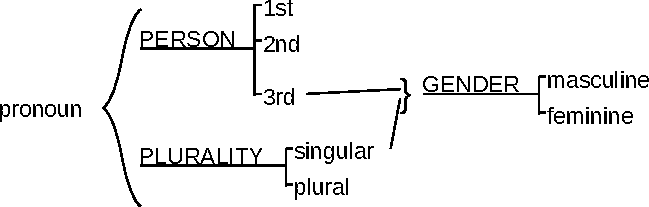
\includegraphics[width=.56\textwidth]{Figures/Example/traditional-pronoun.pdf}      
    \caption{The systematisation of three pronominal features in traditional grammar}
    \label{fig:traditional-pronoun}
\end{figure}

In SFG the pronouns are systematised in the system network of Person from \textit{Introduction to Functional Grammar} \citep[366]{Halliday2013} that is depicted in Figure \ref{fig:person-system-network}. The red rectangles from the figure represent the selections that are applicable to the Subject constituent ``He'' in example above.

\begin{figure}[!ht]
    \centering      
    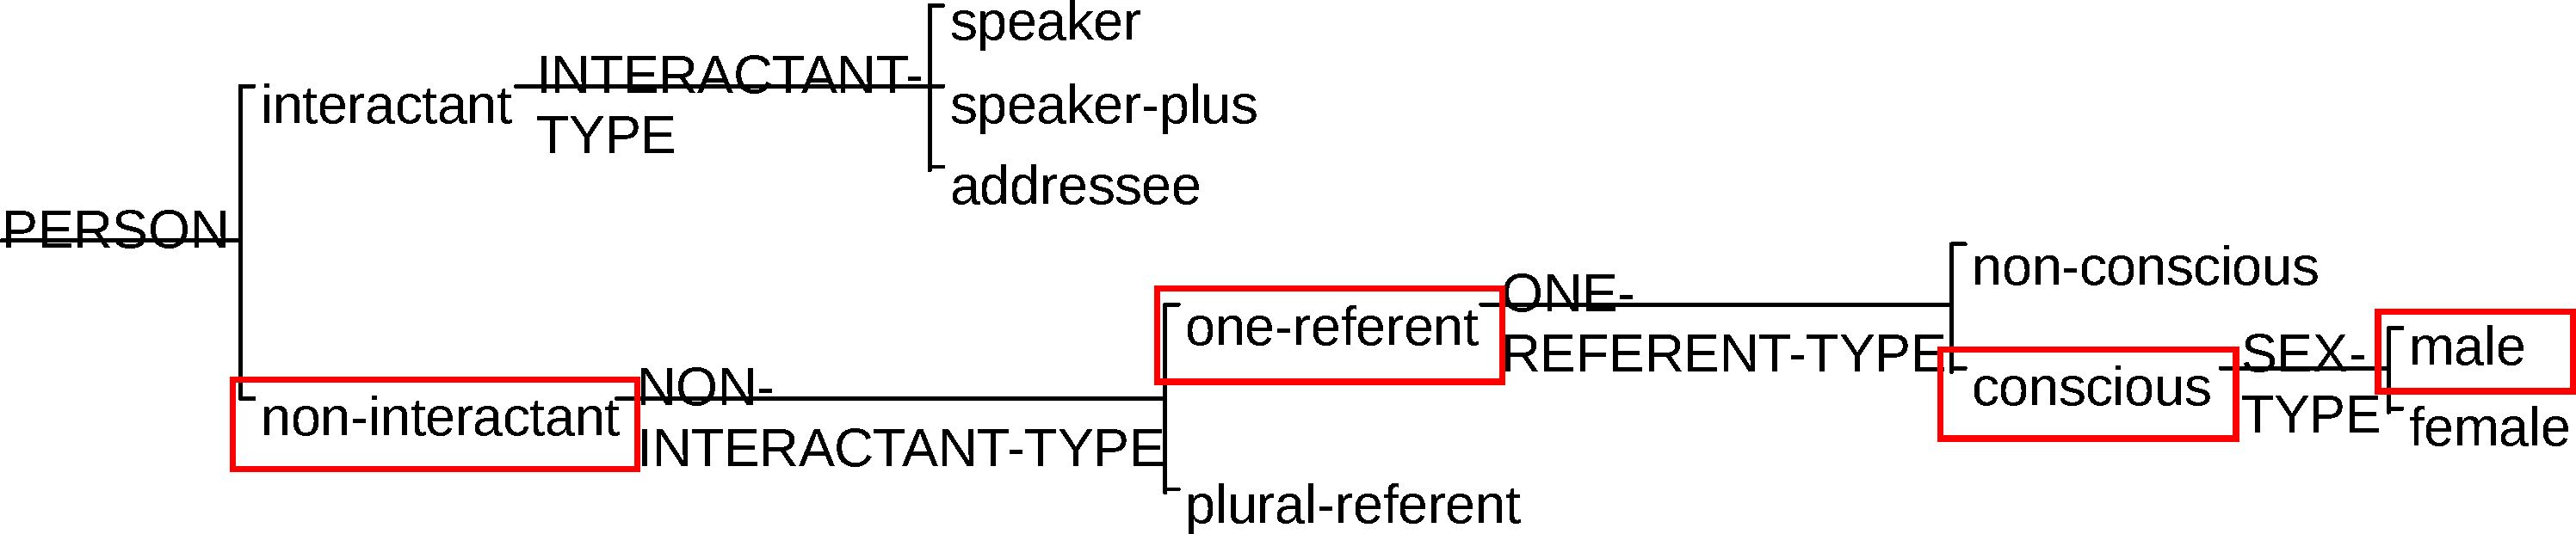
\includegraphics[width=.90\textwidth]{Figures/Example/person-selections.pdf}      
    \caption{The selections in Person system network from \citet[366]{Halliday2013} }
    \label{fig:person-system-network}
\end{figure}

Lets take now the clause constituent that is the root of the constituency tree and see how SFL features can be applied to it. If in in terms of traditional grammar the clause can be ascribed relatively few features i.e. as having \textit{passive voice}, \textit{positive polarity} and \textit{simple past tense} then in terms of SFL grammar the features are many more i.e. \textit{major, positive, active, effective, receptive, agentive, free, finite, temporal, past, non-progressive, non-perfect, declarative, indicative, mood-non-assessed, comment-non-assessed}. Figure \ref{fig:mood-selections} depicts the selections applicable to clause constituent in Example \ref{ex:1} from Mood system network that is an adaptation of Mood network proposed in \citet[162]{Halliday2013}. 

\begin{figure}[!ht]
    \centering      
    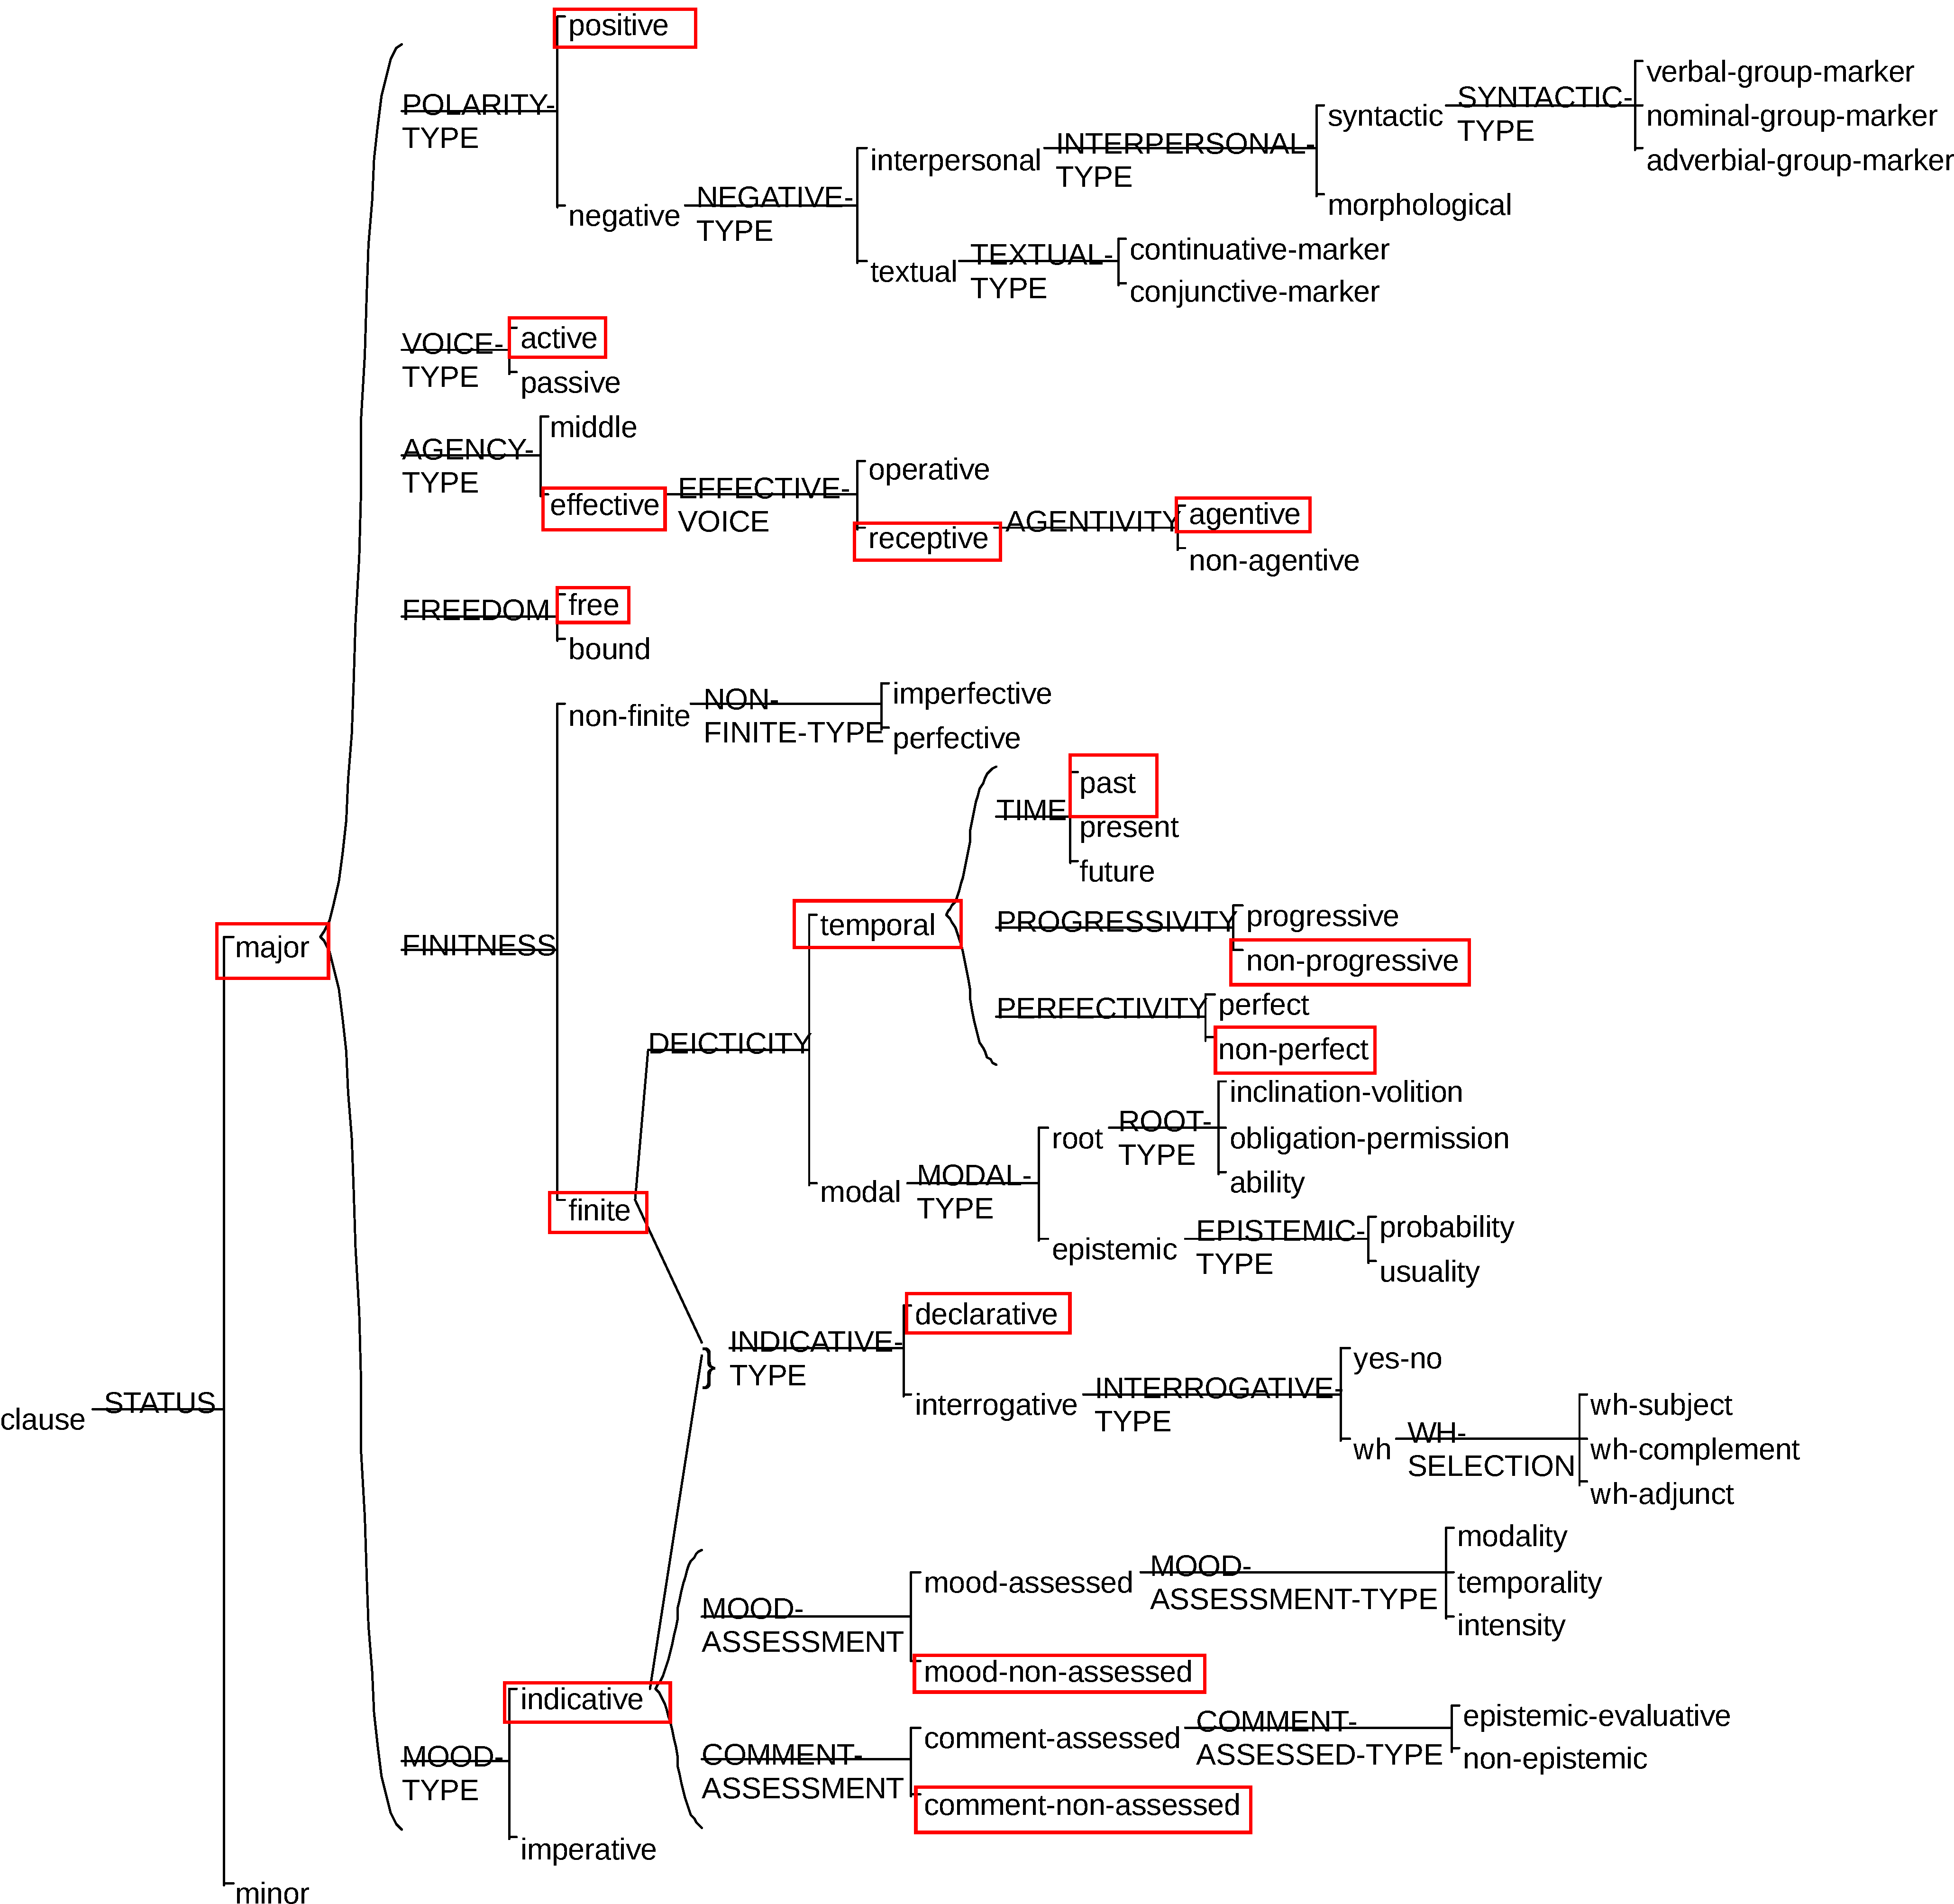
\includegraphics[width=0.91\textwidth]{Figures/Example/mood-selections.pdf}      
    \caption{The systematisation of three pronominal features in traditional grammar}
    \label{fig:mood-selections}
\end{figure}

So far you have seen constituents assigned syntactic functions such as Subject, Complement, Adjunct etc. SFL covers a wider range of functions depending on the kind of meaning it aims at describing. For example what in other grammars is known as \textit{semantic labels}, \textit{thematic} or \textit{$\theta$ roles} SFL systematises as Transitivity system network (which will be introduced in Chapter \ref{sfg} below). Transitivity aims at providing domain independent \textit{semantic frames} called in SFL \textit{process configurations} which describe semantic actions and relationships, along with \textit{semantic roles} ascribed to their \textit{participants}. These semantic frames generally are governed by verbs and more specifically each verb meaning has a dedicated semantic frame. 

For example \ref{ex:1} corresponds to a Possessive semantic frame where ``He'' is the Agent and Carrier whereas ``the cake'' is the Possessed thing as marked in Example \ref{ex:3}. These configurations and participant roles correspond to Transitivity system network proposed in \citep{Neale2002}.

\begin{exe}
    \ex\label{ex:3} [_{Agent-Carrier} He] gave [_{Possessed} the cake] away. 
\end{exe}

There are more functions and features that can be assigned to the constituents in the Example \ref{ex:1} but I stop here. The analysis provided so far highlights that SFG grammar has a variety of functions serving to express different meanings. The traditional grammar distinguishes them as syntactic and semantic functions but, as we will see in Chapter \ref{ch:sfg} below, SFL does not make such a distinction. Another aim of the current section was to provide a glance of the feature rich grammar and I hope the example with Mood feature selection in Figure \ref{fig:mood-selections} fulfils this goal.

\begin{figure}[!ht]
    \centering
    \begin{tikzpicture}[scale=0.8, transform shape, tree-style, 
    level 1/.style={sibling distance=11em, level distance=14em},
    level 2/.style={sibling distance=10em, level distance=12em}, 
    anchor=north
    growth parent anchor = north,]
    
    \node (cla) [pattern-node, split-node, text width = 42em,]  
    {clause 
        \nodepart{two} Configuration
        \nodepart{three} major, positive, active, effective, receptive, agentive, free, finite, temporal, past, non-progressive, non-perfect, declarative, indicative, mood-non-assessed, comment-non-assessed, posessive};
    
    \node (sub) [pattern-node, split-node, below=3em of cla, xshift=-16em,] 
    {pronoun
        \nodepart{two} Subject, Participant,\\ 
        Agent \& Carrier 
        \nodepart{three} 3^{rd} person, singular,\\ 
        male, non-interactant,\\ 
        one-referent, conscious};
    
    \node (mv)[pattern-node, split-node, below=3em of cla, xshift=-5em] 
    {verb
        \nodepart{two} Main Verb, Finite, \\Process 
        \nodepart{three} possessive };
    
    \node (com)[pattern-node,split-node, below=3em of cla, xshift=6em] 
    {nominal group
        \nodepart{two} Complement, Participant, 
        \\ Affected \& Possessed
        \nodepart{three} };
    
    \node (det)[pattern-node,split-node, below=3em of com, xshift=-6em]
    {determiner
        \nodepart{two} Deictic, Modifier
        \nodepart{three} specific, demonstrative,\\ 
        determinative, non-selective};
    
    \node (nou)[pattern-node,split-node, below=3em of com, xshift=6em]
    {noun
        \nodepart{two} Thing, Head
        \nodepart{three} inanimate, singular,\\ 
        countable };
    
    \node[pattern-node,split-node, below=3em of cla, xshift=17em](adjunct)
    {adverb
        \nodepart{two} Adjunct,
        \\Circumstance,
        \\Location
        \nodepart{three} };
    
    \draw[sequence,-,edge-style] (cla.south) -- ++(0,-1em) -| (sub.north);
    \draw[sequence,-,edge-style] (cla.south) -- ++(0,-1em) -| (mv.north);
    \draw[sequence,-,edge-style] (cla.south) -- ++(0,-1em) -| (com.north);
    \draw[sequence,-,edge-style] (cla.south) -- ++(0,-1em) -| (adjunct.north);
    \draw[sequence,-,edge-style] (com.south) -- ++(0,-1em) -| (det.north);
    \draw[sequence,-,edge-style] (com.south) -- ++(0,-1em) -| (nou.north);	
    \end{tikzpicture}
    \caption{Representation of Example \ref{ex:1} as feature rich constituency graph}
    \label{fig:mcg-graph-example}
\end{figure}


Next, Figure \ref{fig:mcg-graph-example} summarises everything discussed above into a partially filled constituency tree. The constituents that were not discussed are assigned only few high level functions and features. As you can see, every node is richly decorated with syntactic and semantic features. The blue part of each node denotes grammatical class, the red part carries functions some of  which are important to establishing a valid constituency structure (that are Mood functions) and the the Transitivity functions; and the green part some grammatical features selected from system networks. In practice, the feature set is much richer than what nodes in Figure \ref{fig:mcg-graph-example} carry here the restriction aims simply to avoid an over-crowded example. 


%Generating automatically feature rich constituency structure such as the one in Figure \ref{fig:mcg-graph-example} is the general aim in the current work.

Next I describe what opportunities and limitations exist in automatically generating rich SFL analyses as until now it has not been possible to use these detailed analysis in computational contexts. This makes them unavailable for corpus work, for training data in machine learning and other end-user application scenarios provided as motivation in the Sections \ref{sec:motivation} and \ref{sec:motivation-business} above.

\section{The problem of parsing with SFGs}
\label{sec:problem}

%\todo[inline]{
%    But, until now it has not been possible to use these
%    detailed analysis in computational contexts: this makes
%    them unavailable for corpus work, for training data in
%    machine learning, etc. etc. (add as many points as occur
%    to you).
%}

%\todo[inline]{
%    There have been attempts to make this work (which you
%    will come back to and describe in Chapter X in detail), however,
%    but these have not worked. As you you say you will describe in detail
%    in Chapter X, }

%\todo[inline]{
%    there is however a strong diagnostic as to
%    just why these attempts have not been successful: i.e., the
%    lack of structural detail that SFG descriptions typically
%    provide. This is argued in general in Bateman (2008)
%    and Teich (1999) [and any other references you can find].
%}

%The problem of parsing with SFG has been well laid out in \citet{Bateman2008} as being one of computational complexity due to exponential explosion of possible combinations of features. 

SFL since it has been established has been primarily concerned with the paradigmatic axis of language. Accounts of the syntagmatic axis of language, for example syntactic structure, have been put in the background. The structure has been placed on the theoretical map and defined in terms of rank, unit, class and function, as we will see in detail in Chapter \ref{ch:sfg} but afterwards it received minimal attention as most of the focus was on the paradigmatic organisation in language (in fact this is is the feature that sets SFL apart from other approaches to study language). This has led to progress in accounting how language works at all strata but little was said about the language constituency. And this can be considered ``unsolved'' within SFL accounts leaving a ``gap in what must be one the central areas of any characterisation of language'' \citep[25]{Bateman2008}. 

%As we will see below, some accounts of constituency are provided within SFL grammars, enough even to make them applicable in computational domains such as automatic \textit{natural language generation}. But such descriptions are by far not satisfiable with respect to what would a proper syntagmatic account of language would be. 

This may be surprising as the syntagmatic dimension is implicit and present everywhere in the SFL literature. For instance all example analyses in the \textit{Introduction to Functional Grammar} \citep{Halliday2013} are predominantly syntagmatic. Moreover, Robin Fawcett for decades promotes the motto \textit{no system network without realisation statements} \citep[9]{Fawcett88-good}. \citet{Bateman2008} presents in detail why there is a severe imbalance between syntagmatic and paradigmatic axes in SFL, how it came to be this way and how it is especially damaging to the task of automatic text analysis. Next I describe the main problems and hint at how potential solutions may look like (for a full account of the solution persuaded in this thesis see Chapter \ref{ch:architecture}). 

\citet{ODonnell2005} offer a detailed description to the long history of SFL being applied in computational contexts yielding with productive outcomes on language theorising, description and processing. The transfer between SFL and computation typically involved a delay between the theoretical formulation and the computational instantiation of that formulation \citep[139]{BatemanMatthiessen88} \citep[19]{MatthiessenBateman91}. The theoretically formulated ideas contain hidden pitfalls that are revealed only upon explicit formulations required by in computation \citep[27]{Bateman2008}. 

The active exchange between the SFL theory and computation has been almost entirely oriented towards automatic \textit{natural language generation}. Such systems would use abstract semantic specifications and communicative goals to produce grammatically correct and well connected texts achieving those goals. This area has been shown to be successful in part due to decomposition of language along the paradigmatic axis using functionally motivated sets of choices between functionally motivated alternatives \citep{McDonald80}.

The computational processes driving the natural language generation relied heavily on the notion of \textit{search}. A well defined search problem is defined in terms of a precise description of the search space which then helps navigation process effectively to find solutions. The paradigmatic organization of the \textit{lexicogrammar} as system networks (that is in SFL the combination of grammar and lexis explained in Section \ref{sec:wording} below) assumed within SFL turns out to organise the search space for possible grammatical units appropriate for communicative goals in almost ideal manner \citep[28]{Bateman2008}.

The \textit{automatic analysis} or \textit{parsing} can be seen as a reverse problem of finding appropriate analysis within a search space of possible solutions. That is identify the exact meaning, systematised in the grammar, of a given natural language sentence. As seen in Section \ref{sec:example} above, an account of the sentence meaning would have to provide both, in terms of a formal structure of the sentence revealing the constituents plus their syntactic relations to each other, and in terms of a complete set of features (detailed to the extent that grammar permits) applicable to each constituent of structure. If, in the generation process, the abstract semantic specifications are increasingly materialised through choice making by traversing the system network towards finally generated text, then, in the parsing process, the reverse is the case. The process starts from a given sentence aiming to derive/search the feature choices in the system network afferent to each of the constituents. But if the paradigmatically organised lexicogrammatical resource is effective for generation it turns out, as we will see next, to be by far unsuitable for the analysis task because of the \textit{size problem}. Halliday himself mentions this problem when he asks \textit{how big is a grammar?}.

\begin{quotation}
    Given any system network it should in principle be possible to count the number of alternatives shown to be available. In practice, it is quite difficult to calculate the number of different selection expressions that are generated by a network of any considerable complexity \citep[10]{Halliday96-grammatics}.
\end{quotation}

The issue emerges from the way connections and (cross-)classifications are organised in a system network. In addition to that, the orientation of systemic grammars towards choice means that the grammar full of disjunctions leading to the problem of search complexity. Also the abstract nature of systemic features leads to a structural richness that adds logical complexity to the task \citep{ODonnell1993}. So estimating the size of the grammar would in fact mean estimating the potential number of feature combinations. For example, a hypothetical network of 40 systems the ``size of the grammar it generates lies somewhere between 41 and 2^{40} (which is somewhere around 10^{12})'' \citep[28]{Bateman2008}. However it is not easy to predict where would the upper limit of the grammar would fall even when the configuration of relations of a particular system network is known.

For the generation task, that size, is not a problem at all as the number of choice points is actually rather small. Such a paradigmatic organisation is, in fact, an incredibly concise and efficient way to express the linguistic choices where the possible feature selections are relevant only when they are enabled by prior paradigmatic choices and it is only those alternatives that need to be considered \citep[12--13]{Halliday96-grammatics} .

In the analysis task, the paradigmatic context of choice, that helps navigation during the generation process, is no longer available. It is not known
any longer which features of a systemic network are relevant and which are not. This leads to a radical asymmetry between the two tasks. That
is: in generation, the simple traversal of the network finds only the compatible choices
because that is what the network leads to; whereas in analysis it is not evident in
advance which path to follow therefore the task is virtually to explore entire search
space in order to discover which features apply to the text. This means that any path is potentially relevant and shall be passed and checked leading to evaluation of the system network as a whole; and that there is no way to restricting the search space, as in the case of generation, to a a set of familiar paradigmatic lines \citep[29]{Bateman2008}. 

One of the grammars successfully used in generation tasks is Nigel grammar developed within Penman generation project \citep{Mann83}. It contains 767 grammatical systems defined over 1381 grammatical features which Bateman evaluates as ``a very large computational grammar by current standards, although nowadays by no means the broadest when considered in terms of raw grammatical coverage'' \citep[29]{Bateman2008}. To parse with such a grammar would means exploring an incredibly vast search space $ 3 \times 10^{18} $ to be more precise. A more detailed break down the complexity by rank or primary class as provided in Table \ref{tab:size} below.

\begin{table}[!ht]
    \centering
    \begin{tabular}{|l|r|}
        \hline
        \textit{rank or primary class} & \textit{size}                             \\ \hline
        adverbial-group                & 18                                        \\ \hline
        words                          & 253                                       \\ \hline
        quantity-group                 & 356                                       \\ \hline
        prepositional-phrase           & 744                                       \\ \hline
        adjectival-group               & 1045                                      \\ \hline
        nominal-group                  & \textgreater $ 2\times 10^{9} $  \\ \hline
        clause                         & \textgreater $ 3\times 10^{18} $ \\ \hline
    \end{tabular}
    \caption{Size of major components of the Nigel grammar expressed in terms of the number of selection expressions generated \citep[35]{Bateman2008}}
    \label{tab:size}
\end{table}

%difficulty SLR
Another difficulty in parsing with SFGs lays in the fact that, as the analysis moves away from directly observable grammatical variations towards more abstract semantic variations, the difficulty of generating an accurate account increases drastically. Transitivity system network for example is made up of such semantic features and it is comparable to what is called in computational linguistics (shallow) \textit{semantic parsing}.

The main challenges (well explained in \citep[245--250]{gildea2002automatic}) in here remains the same since \citet{Winograd1972} that is moving away from the domain specific, hand-crafted semantic specifications towards domain independent and robust set of semantic specifications. This goal was undertaken in several projects to build large broad-scope lexico-semantic databases such as WordNet \citep{Fellbaum98-wn}, FrameNet \citep{Baker1998, Johnson2000, fillmore2003background} and VerbNet \citep{schuler2005verbnet, Kipper2008}. A similar database exists for Transitivity system network as described in \citet{Fawcett2009} called Process Type Database \citep{Neale2002}. 

Such databases describe domain independent \textit{semantic frames} (know in SFL as \textit{configurations} or \textit{figures}) which describe semantic actions and relationships, along with \textit{semantic roles} ascribed to their \textit{participants}. The semantic frames generally are governed by verbs and more specifically each verb meaning has a dedicated semantic frame. For instance the perception frame contains \textit{Perceiver} and \textit{Phenomenon} roles as can be seen in Example \ref{ex:glance1}. 

\begin{exe}
    \ex\label{ex:glance1} [_{Agent-Perceiver} Jaqueline] glanced [_{Phenomenon} at her new watch].
\end{exe}

The tendency is to identify frames that are generic enough to cover classes of verb meanings (for example Action, Cognition, Perception, Possession frames) and the same applies to participant roles where the tendency is to reuse roles across semantic frames (for example agent role from Action frame is reused in Perception or Possession frames, or Phenomenon is reused in Cognition and Perception frames).

%example of covert constituents
Besides being difficult to pin them down in text, the problem with semantic features goes even step further. Sometimes the semantic roles correspond to constituents that are displaced or not even realised in the text which makes them even more difficult to identify and correctly assign. Consider Example \ref{ex:glance2}. It is a sentence that has three non-auxiliary verbs: seem, worry and arrive. According to Cardiff grammar this corresponds to three clauses as represented in Table \ref{tab:three-clauses} below.

%todo continue example

% seem: Attributive: Ca + At
% worry about: two role cognition: Ag Cog + Ph
% miss: possessive : Af Ca + Pos

\begin{exe}
    \ex\label{ex:glance2} She seemed to worry about missing the river boat.
\end{exe}



% concluding problem
Now the question would be how could the vast search space of grammars such as Nigel be restricted to a reasonable size and how can be compensated the lack of proper syntagmatic description in SFGs? The first part of the question has already been addressed in \citet{ODonnell1993} but the lack for an answer to the second part and probably for other hidden reasons the results are not usable in real world applications. In fact the have been more attempts, \citet{Kasper1988}, \citet{Kay1985}, \citet{ODonoghue1991a}, \citet{ODonnell1993} and \citet{Day2007}, to mention just a few, none of which managed to parse broad coverage English with full SFG without aid of some sort. Each had to accept limitations either in grammar or language size and eventually used simpler syntactic trees as a starting point of the parsing process. A detailed account of the current state of the art in parsing with SFGs is provided in Chapter \ref{ch:sota}. 



\section{The problem of semantic parsing}
\label{sec:semantic-parsing-problem}
%todo move upwards and explain as minor problem? 

%As the analysis moves away from directly observable grammatical variations towards more abstract semantic variations the difficulty of generating an accurate account increases drastically. In computational linguistics this area is known as \textit{semantic parsing}. One of the main challenges (well explained in \citep[245--250]{gildea2002automatic}) in  here remains the same since \citet{Winograd1972} that is moving away from the domain specific, hand-crafted semantic specifications towards domain independent and robust set of semantic specifications. This goal was undertaken in several projects to build large broad-scope lexico-semantic databases such as WordNet \citep{Fellbaum98-wn}, FrameNet \citep{Baker1998, Johnson2000, fillmore2003background} and VerbNet \citep{schuler2005verbnet, Kipper2008}.

%Such databases describe domain independent \textit{semantic frames} which describe semantic actions and relationships, along with \textit{semantic roles} ascribed to their participants. The semantic frames generally are governed by verbs and more specifically each verb meaning has a dedicated semantic frame. For instance the perception frame contains \textit{Perceiver} and \textit{Phenomenon} roles as can be seen in Example \ref{ex:glance}. 
%
%\begin{exe}
%    \ex\label{ex:glance} [_{Agent-Perceiver} Jaqueline] glanced [_{Phenomenon} at her new watch].
%\end{exe}
%
%The tendency is to identify frames that are generic enough to cover classes of verb meanings (for example Action, Cognition, Perception, Possession frames) and the same applies to participant roles where the tendency is to reuse roles across semantic frames (for example agent role from Action frame is reused in Perception or Possession frames, or Phenomenon is reused in Cognition and Perception frames).

Semantic role labelling, as motived in \citep[246]{gildea2002automatic}, can play an important role in word sense disambiguation, information extraction, question answering, semantic dialogue systems, machine translation, automatic text summarisation.

%A shallow semantic interpreter operates in terms of domain independent \textit{semantic frames} which describe semantic actions and relationships, along with \textit{semantic roles} ascribed to their participants. 

%Most successful semantic role labelling systems today \citep{he2017deep} are built statistical or (deep) machine learning algorithms training on annotated corpora and incorporating lexical-semantic databases mentioned above. Some stress the importance of syntactic information \citep{punyakanok2008importance} whereas others show good results without \citep{he2017deep}.
%
%In SFL this sort of semantic information is well described in the Transitivity system of the grammar systematising the semantic frames (called \textit{figures} or \textit{configurations}) and the participant roles (called simply \textit{participants}). There is also a lexical-semantic resource called Process Type Database (PTDB) \citep{Neale2002}


\section{On theoretical compatibility and reuse}
\label{sec:reuse}
% reuse motivation, context to parsing 
In the past decades many significant progresses have been made in natural language parsing framed in one or another linguistic theory each adopting a distinct perspective and set of assumptions about language. The theoretical layout and the available resources influence directly what is implemented into the parser and each implementation approach encounters challenges that may or may not be common to other approaches in the same or other theories. 

Parsers implementing one theoretical framework may face common or different problems to those implementing other theories. The same can be said of the solutions. When a solution is achieved using one theory it is potentially reusable in others. The successes and achievements in any school of thought can be regarded as valuable cross theoretical results to the degree links and correspondences can be established. Therefore reusing components that have been shown to work and yield ``good enough results'' is a strong pragmatic motivation in the present work.

%
This thesis employs three linguistic frameworks namely the \textit{Systemic Functional Linguistics}, \textit{Dependency Grammar} and \textit{Governance \& Binding Theory}. SFL has already been motivated in Section \ref{sec:framework} and is introduced in detail in Chapter \ref{ch:sfl}. The other two frameworks are employed because some of the accomplishments using them are directly reused in this thesis and I explain below how. Chapter \ref{ch:dependecy-grappamr} and \ref{ch:gbt} besides introducing the Dependency grammar and correspondingly Government and Binding Theory show how these frameworks relate to each other and to which degree they are compatible to undergo a conversion process for the purpose of reuse.

%The compatibility
%It demonstrates how selected grammatical frameworks namely \textit{Systemic Functional Grammar}, \textit{Dependency Grammar} and \textit{Governance \& Binding Theory} relate to each other and to which degree they are compatible to undergo a conversion process and to show that simple patterns carrying grammatical information can be used to enrich syntactically and semantically the parse structures. And here is a brief motivation for selecting these frameworks.   

%
In the last years \textit{Dependency Grammar} \citep{Tesniere2015} became quite popular in natural language processing world favoured in many projects and systems. The grammatical lightness and the  modern algorithms implemented into dependency parsers such as Stanford Dependency Parser \citep{Marneffe2006}, MaltParser \citep{Nivre2006}, MSTParser \citep{McDonald2006} and Enju \citep{Miyao2005} are increasingly efficient and highly accurate. Among the variety of dependency parsing algorithms, a special contribution bring the \textit{machine learning} methods such as those described in \citet{mcdonald2005online, mcdonald2006online, carreras2007experiments, zhang2011transition, pei2015effective} to name just a few. 

As the dependency parse structures provide information about functional dependencies between words and grants direct access to the predicate-argument relations and can be used off the shelf for real world applications. 
This information alone, would makes the dependency grammar a suitable candidate to supplement the syntagmatic account missing in SFGs and provide some functional hooks for reducing complexity in parsing with SFGs. Hence once of the goals in this work is investigating to which degree the dependency grammar is structurally and functionally compatible with SFGs to undergo a cross theoretic transformation. This hypothesis is theoretically investigated in Chapter \ref{ch:dependecy-grammar} and then evaluate empirically in Chapter \ref{ch:evaluation}. The investigation is based specifically on Stanford Dependencies parser version 3.5 \citep{Marneffe2008a,Marneffe2008, Marneffe2014}. 

\todo{to be continued for GBT}

\section{Thesis Goal and Proposed Solution}

%todo: move towards potential solution

The first difficulty that needs to be addressed, in the analysis process, is discovering from a sequence of words what possible groups are combinable into grammatical groups, phrases or clauses. This is a task of bridging a sequence of words as input and the grammatical description of how they can combine to form a (syntactic) structure (known in SFL as \textit{syntagmatic organizations} and described in Section \ref{sec:structure-sydney}) can already partition the search space into relevant network sub-parts cutting down the complexity by a large factor. Moreover if the syntagmatic account would involve \textit{configurations of grammatical functions} (see Section \ref{sec:functions-metafunctions}) then these grammatical functions can serve as paradigmatic context (similar to the one available during generation task) for traversing the system network and extend to the full set of systemic features. This sort of description can restrict the search space to applicable network parts and provide to an extent traversal context during analysis task.

Addressing the gap of the syntagmatic account within the SFG framework, can be done by, first, providing information about which grammatical functions operate at each rank, second which grammatical functions can be filled by which classes of units and third by providing relative and absolute account of ordering within each unit structure. This sort of information can guide the building of a constituency backbone structure. As a second stage, as mentioned above, the unit classes and grammatical functions can operate as ``hooks'' on system network to guide the traversal in the same way the paradigmatic context available in the generation process. 

Alternatively the problem of structure construction can be outsourced for parsing with other grammars. Then the problem changes into creating a transformation mechanism to obtain the SFL constituency structure rather than build it from scratch. Starting the SFG parsing process from a syntactic tree produced with other grammars reduces the computational complexity of the task and reduce the search space. 

The second stage of constituent enrichment by network traversal can be further aided by checking an arbitrary set of patterns for preselecting even more features recoverable via lexico-syntactic patterns. The pattern recognition plays an essential role in current parsing method for fleshing out the constituent backbone with systemic selections.


\todo[inline]{I Reuse the structural account from other theories}
\todo[inline]{
    Your proposed solution to this problem, and the goal of the thesis,
    is therefore to add some more structural information to a
    complete augmented SFG account by drawing on frameworks which
    have demonstrated coverage of structural detail and which
    also have supported computational instantiation. This will
    be shown and evaluated in the thesis.}

\todo[inline]{
    Reuse structural accounts from other theories that have shown to work well computationally.
Could use famous Chomskyan approach but will use it latter for a more specific problem, that of finding covert constituents (give example of null subject in embedded clause). Instead I turn to Dependency Grammar that increasingly gained popularity in the last 15 years. It has been shown to be computationally fast and it is compatible in many ways with SFG which I will show latter how (mapping DG to SFG). }

\todo[inline]{how: (1) by aligning the primitives and drawing cross-theoretical bridges (see section X), (2) then by mapping grammars (see section Y), (3) implemented using graph transformations (see section Z)}

\todo[inline]{II Enrich the constituency structure with features (since the original goal is to have rich language analysis), that in traditional sense are spanning from purely syntactic (such as tense, voice, case, gender, number etc.) or more semantic or even pragmatic (such as semantic role labels, speech acts, sentiment and appraisal and others) }

\todo[inline]{how: (1) by mapping structure to features (SFL Mood) (see section X), (2) by mapping lexical-semantic resources to fragments of syntactic structure and lexis (lexis contextualised by syntactic structure) (SFL Transitivity) (see section Y), (3) implemented by graph pattern matching (see section Z)}

\todo[inline]{
    So, the thesis goal and outline will be to (and you list them
    explicitly like this too):\newline
    - characterise SFL in its two major variants\newline
    - characterise the previous attempts to parse with SFL and their problems\newline
    - set out two further linguistic frameworks which (a) have\newline
    strong accounts of structural relationships, (b) have shown
    themselves supportive of computational instantiation, and (c) can
    be shown to exhibit suggestive theoretical/descriptive
    links with SFG: in particular, DG and GB.
    
    Chapter X does this for DG
    Chapter Y does this for GB.}


\section{Provisional Thesis Structure}
\todo[inline]{
    1: introduction \\
    2: SFG parsing problem (simple explanation) and SOTA \\
    3: Architecture presentation, introducing challenges of every step and make future references, also the structure of the thesis. \\
    4: SFL grammar \\
    5: Dep Grammar \\
    5: GBT (has to stay here somehow) \\
%    6: the data structures + operations \\ no more data structures, dictribute where needed
    7: the structure creation (introducing basic computer scientific definitions of data structures and other needs) (introducing the exact SFG grammar constituents) \\
    8: the syntactic feature enrichment (introducing basic computer scientific definitions of data structures and other needs) (introducing exact Mood features) \\

    9: the semantic feature enrichment (introducing basic computer scientific definitions of data structures and other needs) (introducing exact Cardiff Transitivity features) \\


    10: Empirical Evaluation \\
    11: Conclusions (what has been achieved and outlook) \\
    
}


\section{References}

[Butler2003] Structure and Function 
[Hjelmslev1953] - Prolegomena-to-a-Theory-of-Language-by-Luis-Hjmeslev
[Elke Teich 1999 ] - Systemic Functional Grammar \& Natural Language Generation - Ch5



\begin{Verbatim}


% feedback Chapter 1 + 2
Dear Eugene,

thanks for file; attached are the detailed comments and corrections and
suggestions for Chapters 1 + 2. I suggest some reorganisation of the
introduction and how the materials in the current chapter 2 are described, you will need to work through the comments to get the
sense of this. But, in short, I think an organisation along the
lines:

Chapter 1: introduction, reasons and goals
Chapter 2: SFG
Chapter 3: State of the Art in approaches to Parsing with SFG and complexity
Chapter 4: DepGrammar
Chapter 5: GBT (perhaps, haven't read these yet)

would get the thesis off to a better start. Also you need to think
about whether all the detail of the SFG variants is important enough
for your task. You will need to provide some more detail of the
organisation of the actual grammars as well in any case, as otherwise
you can't talk about Mood and Transitivity and the like. This is
all clarified in the comments. Alternatively you say very little about
these and introduce them when you get to the later chapters: that
might make sense; I'll see when I get that far. If one went that
road, it would mean not including comments about Mood and Transitivity
in the current chapter 2 though, which might be awkward.

I'll proceed with the other chapters, but as you will see, you have
a fair bit to get going with in any case.

I will not be able to work on the thesis after the end of March. 

theses don't really work like that; so we'll see how far you get.
You (and I) don't want a repeat of the Daniel situation.

Let me know if anything is unclear.

Best,
John.

%feedback Chapter 1 + 2

Dear Eugene,

Comments/corrections for chapters 3 + 4 attached.

Now I'm getting more of a view of the thesis, I'd say that
at present, systemicists will get confused because they'd
wonder why alien things like GB and dependency grammar
appear, and formal/computational linguists would get
confused because they wouldn't be clear why one would
want to take something like SFL. This can be managed
fairly straightforwardly I suspect by setting up the
argument in the Introduction in a clear way, so that
everyone knows just why these things are coming together.
I'd suggest the following kind of outline for the
introduction to make that work, let me know if you
have any problems or questions about this as it
would seem (to me) to be a good way of making all
the bits fits together in a reasonably convincing
fashion. This would also help avoid a reoccurring problem
in your text at the moment, where you frequently want
to talk about things that you have not yet introduced - this
just makes the text confused and impossible to follow (many
examples of this are picked out explicitly in the comments).

So...

Structure the Intro to the thesis more like this:

First, point to the increasing and increasingly recognized
need for deeper, richer semantic/pragmatic analyses across
a broad range of applications: corpora, human-machine
interaction, intelligent interfaces and assistance robotics,
whatever you can find with references supporting the
claim.

Second, a large amount of description of this kind has
traditionally been done, and done a lot, in SFL. Here again
you need to find a good collection of example 'applications'
in SFL (not computational) where the deeper analysis
has been found useful and give references: education,
text/discourse analysis (critical), whatever plus references.

But, until now it has not been possible to use these
detailed analysis in computational contexts: this makes
them unavailable for corpus work, for training data in
machine learning, etc. etc. (add as many points as occur
to you).

There have been attempts to make this work (which you
will come back to and describe in Chapter X in detail), however,
but these have not worked. As you you say you will describe in detail
in Chapter X, there is however a strong diagnostic as to
just why these attempts have not been successful: i.e., the
lack of structural detail that SFG descriptions typically
provide. This is argued in general in Bateman (2008)
and Teich (1999) [and any other references you can find].

You then give EXAMPLES of some difficult cases, where
you illustrate what an SFG analysis would like look and
you point out the lack of structural detail, informally
so that it can be understood directly without further
technical detail. Preferably bringing out some
cases where it is evident that there is no information,
e.g., about raising and control (Teich) and anything
else which would make interpretation difficult.

Your proposed solution to this problem, and the goal of the thesis,
is therefore to add some more structural information to a
complete augmented SFG account by drawing on frameworks which
have demonstrated coverage of structural detail and which
also have supported computational instantiation. This will
be shown and evaluated in the thesis.

So, the thesis goal and outline will be to (and you list them
explicitly like this too):
- characterise SFL in its two major variants
- characterise the previous attempts to parse with SFL and their problems
- set out two further linguistic frameworks which (a) have
strong accounts of structural relationships, (b) have shown
themselves supportive of computational instantiation, and (c) can
be shown to exhibit suggestive theoretical/descriptive
links with SFG: in particular, DG and GB.

Chapter X does this for DG
Chapter Y does this for GB.

- Following this, Chapter Y+1 brings these altogether in a single
architecture (can be short: material from the current introduction
about the system architecture goes here, or can be longer, if
you take the material about merging GB and DG and then with SFG
here too: this might be best).

- rest of chapters go into details.

- Chapter $-1 Evaluation
- Chapter $ What has been achieved and outlook.


I think this kind of explicit form in the Introduction of
the thesis would tell a convincing story that
would make the most of what you currently have and simply wrap
this in a structure that readers can follow and accept. Then
you strengthen the existing bits of text to explicitly draw
attention to these goals as you go so that the reader
remembers where they are and what you are trying to do (and why).
I think this is a fair bit of work still, but relatively
straightforward as it is more about imposing structure and
getting things in the right order. Definitely a thesis in
there struggling to get out! :-)

Best,
John.

%feedback Chapter 5

Hi Eugen,

here is chapter 5 commented. In this one, there are many more
comments about content that will need fixing up, so not just
style of presentation. Many of the problems though come, I suspect,
because you have not yet introduced the algorithm and pipeline
and its datastructures sufficiently that the reader has any
idea what your formalisations here are attempting to do. I think
many of them can just disappear, since you certainly won't
be able to use them anywhere. To define a data structure, you
don't need a full first-order theory, that is overkill. You
do not get any points for formalisation; you'd only get points
for appropriate, necessary and well motivated formalisation,
and many of the definitions in this chapter do not meet
this requirement. You only need as much formalism as necessary
to get the job done. And the job is the task that you need
to have described as the pipeline of the system: probably best
immediately after the discussion of GB. There are many
interesting decisions made in this chapter, but they are
just lost in the mass of probably hardly relevant detail.
So introducing the pipeline and its data structures first,
would give you a better way of picking out just that which
is a crucial contribution of your thesis, i.e., the stuff
that makes parsing work. Providing definitions of
morphisms between graphs does *not* do that; and it is
hardly your job and has been done more or less completely
before in appropriate formal texts in any case.

In short, you need to provide the new architecture and pipeline
chapter and rewrite this one accordingly.

Let me know when that has happened, as that will be the next
major version that it would be sensible for me to comment on
I think. The actual details of the parsing algorithm that
occurs in subsequent chapters will I hope be more straightforward,
once the groundwork is out of the way.

Best,
John.

---
Am 08.03.18 um 22:00 schrieb Eugen Costezki:
> I wanted to say that this chapter 5 represented a special kind of struggle  as I was tempted to define entire computer science.

yes, I noticed! :-) Fortunately, you do not need to do this...
so simplifications are ahead!

Best,
John

\end{Verbatim}